% questions.tex —— 2015 年·湖南卷·理科 · 题目内容片段（无答案）
% 由 tools/generate_projects.py 依来源总账自 2015/2015_数学真题_湖南理_试题.md 生成，勿手改（改源 MD 后重跑）

\begin{gktip}
来源：固定 PDF 普通高考/2015/2015湖南理.pdf（SHA-256 见来源校对记录）。原卷为 A3 横向双页排版，印刷页码 955–956。PDF 本身没有答案页；本文件仅转录题面，不含推导答案。图形/表格状态见同目录图形清单：五处图形已有 TikZ 矢量草稿，Q12 茎叶图以 LaTeX 表格转录；尚待正式版本排版和页校。
\end{gktip}

\gkpart{一、选择题}

\begin{question}
\gkti{1}

已知 \(\dfrac{(1-i)^2}{z}=1+i\)（\(i\) 为虚数单位），则复数 \(z=\)（　）

(A) \(1+i\)　(B) \(1-i\)　(C) \(-1+i\)　(D) \(-1-i\)

\end{question}
\begin{question}
\gkti{2}

设 \(A,B\) 是两个集合，则“\(A\cap B=A\)”是“\(A\subseteq B\)”的（　）

(A) 充分不必要条件　(B) 必要不充分条件　(C) 充要条件　(D) 既不充分也不必要条件

\Needspace{0.4\textheight}
\end{question}
\begin{question}
\gkti{3}

执行如图所示的程序框图，如果输入 \(n=3\)，则输出的 \(S=\)（　）。
\nopagebreak[4]
\begin{center}% Source: fixed 2015 Hunan science paper, printed page 955.
% Vector redraw from the source diagram; not a raster crop.
\begin{tikzpicture}[>=stealth, every node/.style={font=\fontsize{10.5pt}{12.6pt}\selectfont, inner sep=3pt}]
  \node[draw, rounded corners] (start) at (0,0) {开始};
  \node[draw, trapezium, trapezium left angle=70, trapezium right angle=110, below=7mm of start] (input) {输入 $n$};
  \node[draw, rectangle, below=7mm of input] (init) {$i=1,\ S=0$};
  \node[draw, rectangle, text width=48mm, align=center, below=7mm of init] (sum) {$S=S+\dfrac{1}{(2i-1)(2i+1)}$};
  \node[draw, rectangle, below=7mm of sum] (inc) {$i=i+1$};
  \node[draw, diamond, aspect=2.2, below=7mm of inc] (test) {$i>n?$};
  \node[draw, trapezium, trapezium left angle=70, trapezium right angle=110, below=7mm of test] (output) {输出 $S$};
  \node[draw, rounded corners, below=7mm of output] (end) {结束};
  \draw[->] (start) -- (input);
  \draw[->] (input) -- (init);
  \draw[->] (init) -- (sum);
  \draw[->] (sum) -- (inc);
  \draw[->] (inc) -- (test);
  \draw[->] (test) -- node[right, inner sep=2pt] {是} (output);
  \draw[->] (output) -- (end);
  \coordinate (loopright) at ($(test.east)+(13mm,0)$);
  \draw (test.east) -- (loopright |- test.east) -- (loopright |- sum.east);
  \draw[->] (loopright |- sum.east) -- (sum.east);
  \node[right, inner sep=2pt] at ($(loopright |- test.east)!0.55!(loopright |- sum.east)$) {否};
\end{tikzpicture}
\end{center}
\nopagebreak[4]
(A) \(\dfrac67\)　(B) \(\dfrac37\)　(C) \(\dfrac89\)　(D) \(\dfrac49\)

\end{question}
\begin{question}
\gkti{4}

\Needspace{5\baselineskip}
若变量 \(x,y\) 满足约束条件
\nopagebreak[4]
\[
\begin{cases}
x+y\geqslant -1,\\
2x-y\leqslant 1,\\
y\leqslant 1,
\end{cases}
\]
则 \(z=3x-y\) 的最小值为（　）

(A) \(-7\)　(B) \(-1\)　(C) \(1\)　(D) \(2\)

\end{question}
\begin{question}
\gkti{5}

设函数 \(f(x)=\ln(1+x)-\ln(1-x)\)，则 \(f(x)\) 是（　）

(A) 奇函数，且在 \((0,1)\) 是增函数　(B) 奇函数，且在 \((0,1)\) 是减函数

(C) 偶函数，且在 \((0,1)\) 是增函数　(D) 偶函数，且在 \((0,1)\) 是减函数

\end{question}
\begin{question}
\gkti{6}

已知 \(\left(\sqrt{x}-\dfrac{a}{\sqrt{x}}\right)^5\) 的展开式中含 \(x^{\frac32}\) 的项的系数为 \(30\)，则 \(a=\)（　）

(A) \(\sqrt3\)　(B) \(-\sqrt3\)　(C) \(6\)　(D) \(-6\)

\Needspace{0.4\textheight}
\end{question}
\begin{question}
\gkti{7}

在如图所示的正方形中随机投掷 \(10000\) 个点，则落入阴影部分（曲线 \(C\) 为正态分布 \(N(0,1)\) 的密度曲线）的点的个数的估计值为（　）

\Needspace{5\baselineskip}
附：若 \(X\sim N(\mu,\sigma^2)\)，则
\nopagebreak[4]
\[
P(\mu-\sigma<X\leqslant\mu+\sigma)=0.6826,\qquad
P(\mu-2\sigma<X\leqslant\mu+2\sigma)=0.9544.
\]
\nopagebreak[4]
\begin{center}% Source: fixed 2015 Hunan science paper, printed page 955.
% Exact standard-normal density on [0,1], matching the unit-square diagram.
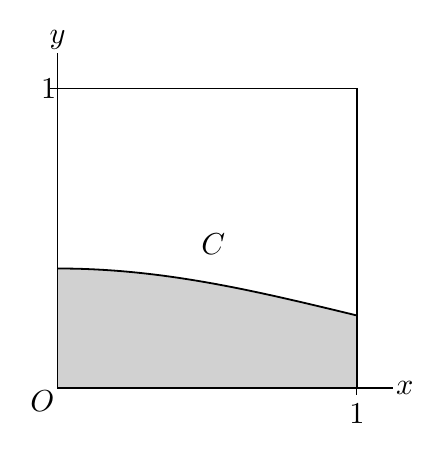
\begin{tikzpicture}[x=38mm,y=38mm, every node/.style={font=\fontsize{10.5pt}{12.6pt}\selectfont, inner sep=1pt}]
  \path[fill=black!18] (0,0) -- plot[domain=0:1,samples=80] (\x,{exp(-\x*\x/2)/sqrt(2*pi)}) -- (1,0) -- cycle;
  \draw[line width=.45pt] (0,0) -- (1.12,0) node[right] {$x$};
  \draw[line width=.45pt] (0,0) -- (0,1.12) node[above] {$y$};
  \draw[line width=.45pt] (0,0) rectangle (1,1);
  \draw[line width=.65pt,domain=0:1,samples=80] plot (\x,{exp(-\x*\x/2)/sqrt(2*pi)});
  \draw (1,.025) -- (1,-.025) node[below=2pt] {$1$};
  \draw (-.025,1) -- (.025,1) node[left=2pt] {$1$};
  \node at (.52,.48) {$C$};
  \node[below left] at (0,0) {$O$};
\end{tikzpicture}
\end{center}
\nopagebreak[4]
(A) \(2386\)　(B) \(2718\)　(C) \(3413\)　(D) \(4772\)

\end{question}
\begin{question}
\gkti{8}

已知点 \(A,B,C\) 在圆 \(x^2+y^2=1\) 上运动，且 \(AB\perp BC\)。若点 \(P\) 的坐标为 \((2,0)\)，则 \(\left|\overrightarrow{PA}+\overrightarrow{PB}+\overrightarrow{PC}\right|\) 的最大值为（　）

(A) \(6\)　(B) \(7\)　(C) \(8\)　(D) \(9\)

\end{question}
\begin{question}
\gkti{9}

将函数 \(f(x)=\sin 2x\) 的图象向右平移 \(\varphi\)（\(0<\varphi<\dfrac{\pi}{2}\)）个单位后得到函数 \(g(x)\) 的图象。若对满足 \(\lvert f(x_1)-g(x_2)\rvert=2\) 的 \(x_1,x_2\)，有 \(\lvert x_1-x_2\rvert_{\min}=\dfrac{\pi}{3}\)，则 \(\varphi=\)（　）

(A) \(\dfrac{5\pi}{12}\)　(B) \(\dfrac{\pi}{3}\)　(C) \(\dfrac{\pi}{4}\)　(D) \(\dfrac{\pi}{6}\)

\Needspace{0.4\textheight}
\end{question}
\begin{question}
\gkti{10}

某工件的三视图如图所示，现将该工件通过切削，加工成一个体积尽可能大的长方体新工件，并使新工件的一个面落在原工件的一个面内，则原工件材料的利用率为（材料的利用率 \(=\dfrac{\text{新工件的体积}}{\text{原工件的体积}}\)）（　）
\nopagebreak[4]
\begin{center}% Source: fixed 2015 Hunan science paper, printed page 955.
% The three orthographic views identify a right circular cone; vector redraw.
\begin{tikzpicture}[x=14mm,y=14mm, every node/.style={font=\fontsize{10.5pt}{12.6pt}\selectfont, inner sep=1pt}, every path/.style={line width=.45pt}]
  % Front view
  \draw (0,0) -- (1,2) -- (2,0) -- cycle;
  \draw[<->] (-.22,0) -- (-.22,2) node[midway,left] {$2$};
  \draw[<->] (1,2.22) -- (2,2.22) node[midway,above] {$1$};
  \draw[<->] (0,-.22) -- (2,-.22) node[midway,below] {$2$};
  \node[below=7mm] at (1,0) {正视图};
  % Side view
  \begin{scope}[xshift=3.2cm]
    \draw (0,0) -- (1,2) -- (2,0) -- cycle;
    \draw[<->] (-.22,0) -- (-.22,2) node[midway,left] {$2$};
    \draw[<->] (1,2.22) -- (2,2.22) node[midway,above] {$1$};
    \draw[<->] (0,-.22) -- (2,-.22) node[midway,below] {$2$};
    \node[below=7mm] at (1,0) {侧视图};
  \end{scope}
  % Plan view (diameter 2)
  \begin{scope}[xshift=1.0cm,yshift=-3.8cm]
    \draw (1,1) circle[radius=1];
    \node[below=7mm] at (1,0) {俯视图};
  \end{scope}
\end{tikzpicture}
\end{center}
\nopagebreak[4]
(A) \(\dfrac{8}{9\pi}\)　(B) \(\dfrac{16}{9\pi}\)　(C) \(\dfrac{4(\sqrt2-1)^3}{\pi}\)　(D) \(\dfrac{12(\sqrt2-1)^3}{\pi}\)

\end{question}
\gkpart{二、填空题}

\begin{question}
\gkti{11}

\(\displaystyle\int_0^2(x-1)\,\mathrm dx=\underline{\hspace{2cm}}\)。

\end{question}
\begin{question}
\gkti{12}

\Needspace{5\baselineskip}
在一次马拉松比赛中，35 名运动员的成绩（单位：分钟）茎叶图如图所示。

\nopagebreak[4]
\[
\begin{array}{c|l}
13 & 0\quad0\quad3\quad4\quad5\quad6\quad6\quad8\quad8\quad8\quad9\\
14 & 1\quad1\quad1\quad2\quad2\quad2\quad3\quad3\quad4\quad4\quad5\quad5\quad5\quad6\quad6\quad7\quad8\\
15 & 0\quad1\quad2\quad2\quad3\quad3\quad3
\end{array}
\]

若将运动员按成绩由好到差编为 \(1\sim35\) 号，再用系统抽样的方法从中抽取 7 人，则其中成绩在区间 \([139,151]\) 上的运动员的人数是\gkblank{}。

\end{question}
\begin{question}
\gkti{13}

设 \(F\) 是双曲线 \(C:\dfrac{x^2}{a^2}-\dfrac{y^2}{b^2}=1\) 的一个焦点，若 \(C\) 上存在点 \(P\)，使线段 \(PF\) 的中点恰为其虚轴的一个端点，则 \(C\) 的离心率为\gkblank{}。

\end{question}
\begin{question}
\gkti{14}

设 \(S_n\) 为等比数列 \(\{a_n\}\) 的前 \(n\) 项和，若 \(a_1=1\)，且 \(3S_1,2S_2,S_3\) 成等差数列，则 \(a_n=\)\gkblank{}。

\end{question}
\begin{question}
\gkti{15}

\Needspace{5\baselineskip}
已知函数
\nopagebreak[4]
\[
f(x)=\begin{cases}
x^3,&x\leqslant a,\\
x^2,&x>a,
\end{cases}
\]
若存在实数 \(b\)，使函数 \(g(x)=f(x)-b\) 有两个零点，则 \(a\) 的取值范围是\gkblank{}。

\end{question}
\gkpart{三、解答题}

\Needspace{0.4\textheight}
\begin{question}
\gkti{16}\textbf{三选二} 

以下 A、B、C 三题任选两题作答。

\textbf{【A】} 如图，在 \(\odot O\) 中，相交于点 \(E\) 的两弦 \(AB,CD\) 的中点分别是 \(M,N\)，直线 \(MO\) 与直线 \(CD\) 相交于点 \(F\)。证明：
\nopagebreak[4]
\begin{center}% Source: fixed 2015 Hunan science paper, printed page 955.
% Topological vector redraw; relative positions are schematic, not to scale.
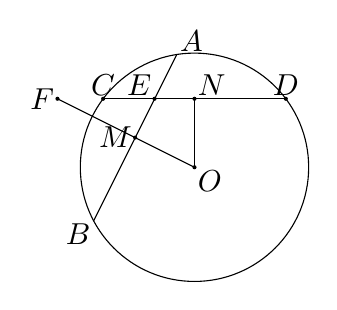
\begin{tikzpicture}[scale=1.45, every node/.style={font=\fontsize{10.5pt}{12.6pt}\selectfont, inner sep=1pt}]
  \coordinate (O) at (0,0);
  \coordinate (C) at (-.8,.6);
  \coordinate (D) at (.8,.6);
  \coordinate (N) at (0,.6);
  \coordinate (E) at (-.35,.6);
  \coordinate (M) at (-.52,.26);
  \coordinate (F) at (-1.20,.6);
  \draw (O) circle[radius=1];
  \draw (C)--(D);
  % Chord AB through E, perpendicular to OM; endpoints lie on the circle.
  \draw (-.883,-.468) -- (-.155,.988);
  \draw (F)--(O);
  \draw (O)--(N);
  \fill (O) circle[radius=.018] (C) circle[radius=.018] (D) circle[radius=.018]
        (E) circle[radius=.018] (M) circle[radius=.018] (N) circle[radius=.018] (F) circle[radius=.018];
  \node[above] at (C) {$C$};
  \node[above] at (D) {$D$};
  \node[above left] at (E) {$E$};
  \node[left] at (M) {$M$};
  \node[above right] at (N) {$N$};
  \node[left] at (F) {$F$};
  \node[below right] at (O) {$O$};
  \node[above right] at (-.155,.988) {$A$};
  \node[below left] at (-.883,-.468) {$B$};
\end{tikzpicture}
\end{center}
\nopagebreak[4]
(1) \(\angle MEN+\angle NOM=180^\circ\)；

(2) \(FE\cdot FN=FM\cdot FO\)。

\textbf{【B】} 已知直线 \(l:\begin{cases}x=5+\dfrac{\sqrt3}{2}t,\\y=\sqrt3+\dfrac12t,\end{cases}\)（\(t\) 为参数），以坐标原点为极点，\(x\) 轴的正半轴为极轴建立极坐标系，曲线 \(C\) 的极坐标方程为 \(\rho=2\cos\theta\)。

(1) 将曲线 \(C\) 的极坐标方程化为直角坐标方程；

(2) 设点 \(M\) 的直角坐标为 \((5,\sqrt3)\)，直线 \(l\) 与曲线 \(C\) 的交点为 \(A,B\)，求 \(\lvert MA\rvert\cdot\lvert MB\rvert\) 的值。

\textbf{【C】} 设 \(a>0,b>0\)，且 \(a+b=\dfrac1a+\dfrac1b\)，证明：

(1) \(a+b\geqslant2\)；

(2) \(a^2+a<2\) 与 \(b^2+b<2\) 不可能同时成立。

\end{question}
\begin{question}
\gkti{17}

设 \(\triangle ABC\) 的内角 \(A,B,C\) 的对边分别为 \(a,b,c\)，\(a=b\tan A\)，且 \(B\) 为钝角。

(1) 证明：\(B-A=\dfrac{\pi}{2}\)；

(2) 求 \(\sin A+\sin C\) 的取值范围。

\end{question}
\begin{question}
\gkti{18}

某商场举行有奖促销活动，顾客购买一定金额的商品后即可抽奖。每次抽奖都是从装有 4 个红球、6 个白球的甲箱和装有 5 个红球、5 个白球的乙箱中，各随机摸出 1 个球。在摸出的 2 个球中，若都是红球，则获一等奖；若只有 1 个红球，则获二等奖；若没有红球，则不获奖。

(1) 求顾客抽奖 1 次能获奖的概率；

(2) 若某顾客有 3 次抽奖的机会，记该顾客在 3 次抽奖中获一等奖的次数为 \(X\)，求 \(X\) 的分布列和数学期望。

\Needspace{0.4\textheight}
\end{question}
\begin{question}
\gkti{19}

如图，已知四棱台 \(ABCD-A_1B_1C_1D_1\) 的上、下底面分别是边长为 3 和 6 的正方形，\(AA_1=6\)，且 \(AA_1\perp\) 底面 \(ABCD\)，点 \(P,Q\) 分别在棱 \(DD_1,BC\) 上。
\nopagebreak[4]
\begin{center}% Source: fixed 2015 Hunan science paper, printed page 956.
% Schematic vector redraw; preserves labeled incidence/hidden-edge topology only.
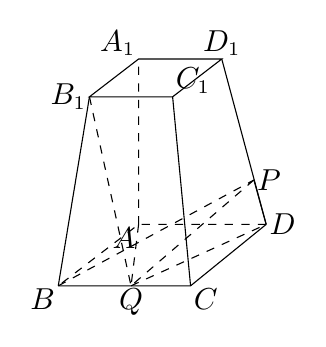
\begin{tikzpicture}[scale=1.2, every node/.style={font=\fontsize{10.5pt}{12.6pt}\selectfont, inner sep=1pt}]
  \coordinate (A) at (0,0);
  \coordinate (B) at (-.85,-.65);
  \coordinate (C) at (.55,-.65);
  \coordinate (D) at (1.35,0);
  \coordinate (Aone) at (0,1.75);
  \coordinate (Bone) at (-.52,1.35);
  \coordinate (Cone) at (.36,1.35);
  \coordinate (Done) at (.88,1.75);
  \coordinate (P) at (1.22,.47);
  \coordinate (Q) at (-.08,-.65);
  % Lower and upper square bases and visible frustum edges.
  \draw (B)--(C)--(D);
  \draw[dashed] (D)--(A)--(B);
  \draw (Bone)--(Cone)--(Done)--(Aone)--cycle;
  \draw (B)--(Bone) (C)--(Cone) (D)--(Done);
  % Hidden edges and the construction segment shown in the source.
  \draw[dashed] (A)--(Aone) (Bone)--(Q) (A)--(Q) (B)--(P) (P)--(Q) (Q)--(D);
  \draw (D)--(P);
  \foreach \pt/\pos/\lab in {A/below left/A,B/below left/B,C/below right/C,D/right/D,
      Aone/above left/A_1,Bone/left/B_1,Cone/above right/C_1,Done/above/D_1,P/right/P,Q/below/Q}
    \node[\pos] at (\pt) {$\lab$};
\end{tikzpicture}
\end{center}
\nopagebreak[4]
(1) 若点 \(P\) 是 \(DD_1\) 的中点，证明：\(AB_1\perp PQ\)；

(2) 若 \(PQ\parallel\) 平面 \(ABB_1A_1\)，二面角 \(P-QD-A\) 的余弦值为 \(\dfrac37\)，求四面体 \(ADPQ\) 的体积。

\end{question}
\begin{question}
\gkti{20}

已知抛物线 \(C_1:x^2=4y\) 的焦点 \(F\) 也是椭圆 \(C_2:\dfrac{y^2}{a^2}+\dfrac{x^2}{b^2}=1\)（\(a>b>0\)）的一个焦点，\(C_1\) 与 \(C_2\) 的公共弦长为 \(2\sqrt6\)。

(1) 求 \(C_2\) 的方程；

(2) 过点 \(F\) 的直线 \(l\) 与 \(C_1\) 相交于 \(A,B\) 两点，与 \(C_2\) 相交于 \(C,D\) 两点，且 \(\overrightarrow{AC}\) 与 \(\overrightarrow{BD}\) 同向。

① 若 \(\lvert AC\rvert=\lvert BD\rvert\)，求直线 \(l\) 的斜率；

② 设 \(C_1\) 在点 \(A\) 处的切线与 \(x\) 轴的交点为 \(M\)，证明：直线 \(l\) 绕点 \(F\) 旋转时，\(\triangle MFD\) 总是钝角三角形。

\end{question}
\begin{question}
\gkti{21}

已知 \(a>0\)，函数 \(f(x)=e^{ax}\sin x\)（\(x\in[0,+\infty)\)），记 \(x_n\) 为 \(f(x)\) 的从小到大的第 \(n\)（\(n\in\mathbb N^*\)）个极值点。证明：

(1) 数列 \(\{f(x_n)\}\) 是等比数列；

(2) 若 \(a\geqslant\dfrac{1}{\sqrt{e^2-1}}\)，则对一切 \(n\in\mathbb N^*\)，\(x_n<\lvert f(x_n)\rvert\) 恒成立。

\end{question}